\documentclass[11pt]{article}

\usepackage[margin=0.8in]{geometry}
\usepackage[utf8]{inputenc}
\usepackage{graphicx}
\usepackage{float}
\usepackage{xcolor}
\usepackage{fancyhdr}
\usepackage{listings}
\usepackage{booktabs}
\usepackage{caption}
\usepackage{hyperref}
\usepackage{titlesec}

\definecolor{darkblue}{RGB}{20,55,95}
\definecolor{lightgray}{RGB}{245,245,245}
\definecolor{codegray}{RGB}{40,40,40}

\pagestyle{fancy}
\fancyhf{}
\lhead{\textbf{ECE 595: AI Infrastructure}}
\chead{\textbf{Homework 3}}
\rhead{\textbf{Scott Nguyen | snguyen9}}
\cfoot{\thepage}
\renewcommand{\headrulewidth}{0.8pt}

\titleformat{\section}
{\large\bfseries\color{darkblue}}
{\thesection}{0.75em}{}

\titleformat{\subsection}
{\normalsize\bfseries\color{darkblue}}
{\thesubsection}{0.75em}{}

\lstdefinestyle{terminal}{
	backgroundcolor=\color{lightgray},
	basicstyle=\ttfamily\small\color{codegray},
	breaklines=true,
	frame=single,
	rulecolor=\color{darkblue},
	columns=fullflexible,
	keepspaces=true
}

\lstdefinestyle{pythoncode}{
	backgroundcolor=\color{lightgray},
	basicstyle=\ttfamily\scriptsize\color{codegray},
	breaklines=true,
	frame=single,
	rulecolor=\color{darkblue},
	columns=fullflexible,
	keepspaces=true,
	language=Python,
	showstringspaces=false
}

\begin{document}
	
	\begin{center}
		{\Large \textbf{Retrieval Augmented Generation with Ollama and LangChain}}\\[0.3em]
		{\large ECE 595: AI Infrastructure}\\[0.3em]
		{\large Scott Nguyen | snguyen9}\\[0.3em]
		{\large Homework 4}
	\end{center}
	
	\vspace{1em}
	
	\section{Introduction}
	
	This assignment implements and evaluates a Retrieval Augmented Generation (RAG) system using a local large language model. The system processes a PDF by splitting it into chunks, embedding the text into a vector database, retrieving relevant context, and generating answers using an Ollama-hosted model.
	
	The implementation uses LangChain utilities, Chroma for vector storage, and HuggingFace embeddings. Experiments were conducted in WSL, and results were recorded for two different RAG configurations.
	
	\section{System Setup}
	
	The system was implemented in Python using a virtual environment in WSL. Two configurations were tested using the following commands:
	
	\begin{lstlisting}[style=terminal, caption={Configuration A run command}]
		python run_questions.py \
		--chunk-size 1200 \
		--chunk-overlap 100 \
		--k 2 \
		--llm llama3.2:latest \
		--output results_config_a.txt
	\end{lstlisting}
	
	\begin{lstlisting}[style=terminal, caption={Configuration B run command}]
		python run_questions.py \
		--chunk-size 500 \
		--chunk-overlap 50 \
		--k 4 \
		--llm llama3.2:latest \
		--output results_config_b.txt
	\end{lstlisting}
	
	\section{RAG Pipeline Design}
	
	The system follows a standard RAG workflow:
	
	\begin{enumerate}
		\item Load the PDF using \texttt{PyPDFLoader}
		\item Split text into chunks with \texttt{RecursiveCharacterTextSplitter}
		\item Generate embeddings using \texttt{all-MiniLM-L6-v2}
		\item Store embeddings in Chroma
		\item Retrieve top-$k$ relevant chunks
		\item Generate responses with a local Ollama model
	\end{enumerate}
	
	\section{Prompt Engineering}
	
	The prompt was designed to force the model to rely only on retrieved document context. The main instruction tells the model to answer from the document and say ``I do not know based on the document'' when the answer is not supported.
	
	This helps reduce hallucinations and makes the system behave more like a document-grounded assistant. The prompt also includes recent conversation history so that the chatbot can respond to limited follow-up questions.
	
	\section{Configuration Comparison}
	
	Two configurations were tested to evaluate how chunk size and retrieval count affect answer quality.
	
	\begin{table}[H]
		\centering
		\caption{RAG Configuration Comparison}
		\begin{tabular}{lcc}
			\toprule
			\textbf{Parameter} & \textbf{Config A} & \textbf{Config B} \\
			\midrule
			Chunk Size & 1200 & 500 \\
			Chunk Overlap & 100 & 50 \\
			Retriever $k$ & 2 & 4 \\
			LLM & llama3.2:latest & llama3.2:latest \\
			Embedding Model & all-MiniLM-L6-v2 & all-MiniLM-L6-v2 \\
			\bottomrule
		\end{tabular}
	\end{table}
	
	Configuration A uses larger chunks and fewer retrieved documents, resulting in faster but less precise retrieval. Configuration B uses smaller chunks and more retrieved results, improving answer quality by increasing relevant context. This shows the trade-off between latency and accuracy.
	
	\section{Terminal Output and Screenshots}
	
	The following screenshots show the system running, building the vector database, and answering automated questions.
	
	\begin{figure}[H]
		\centering
		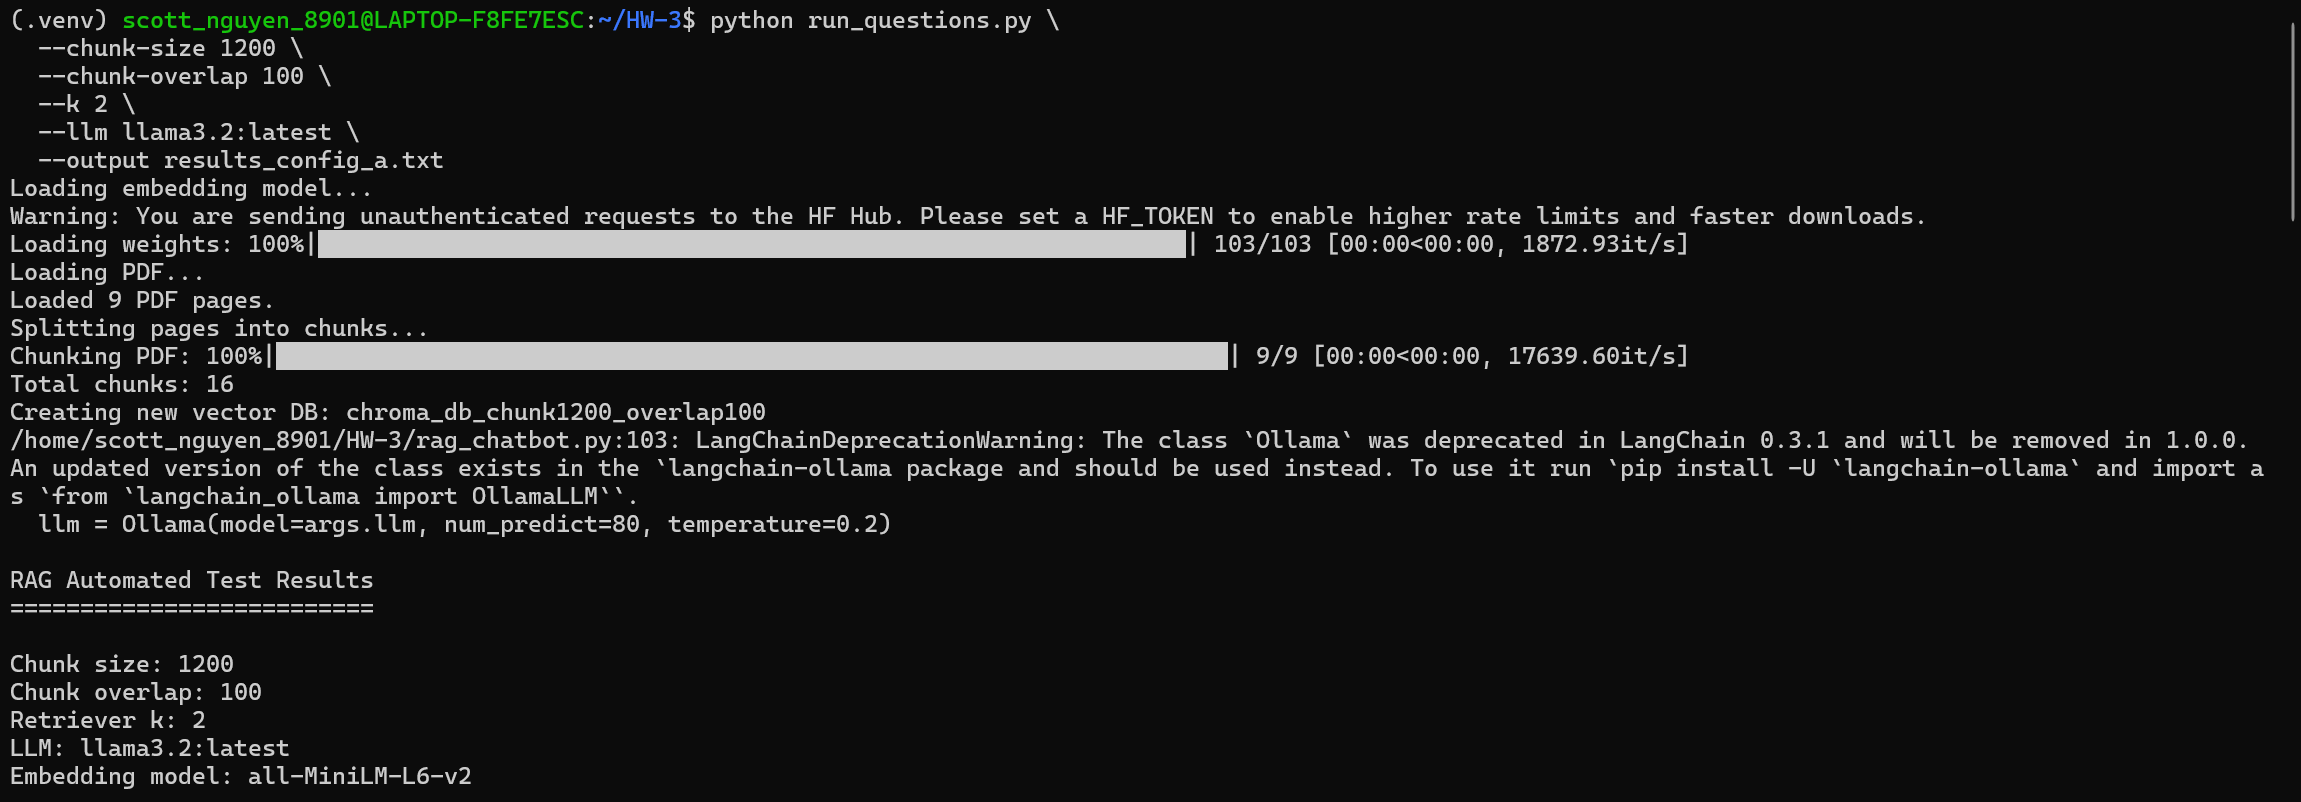
\includegraphics[width=\textwidth]{plots/0.1.png}
		\caption{Configuration A startup and vector database creation.}
	\end{figure}
	
	\begin{figure}[H]
		\centering
		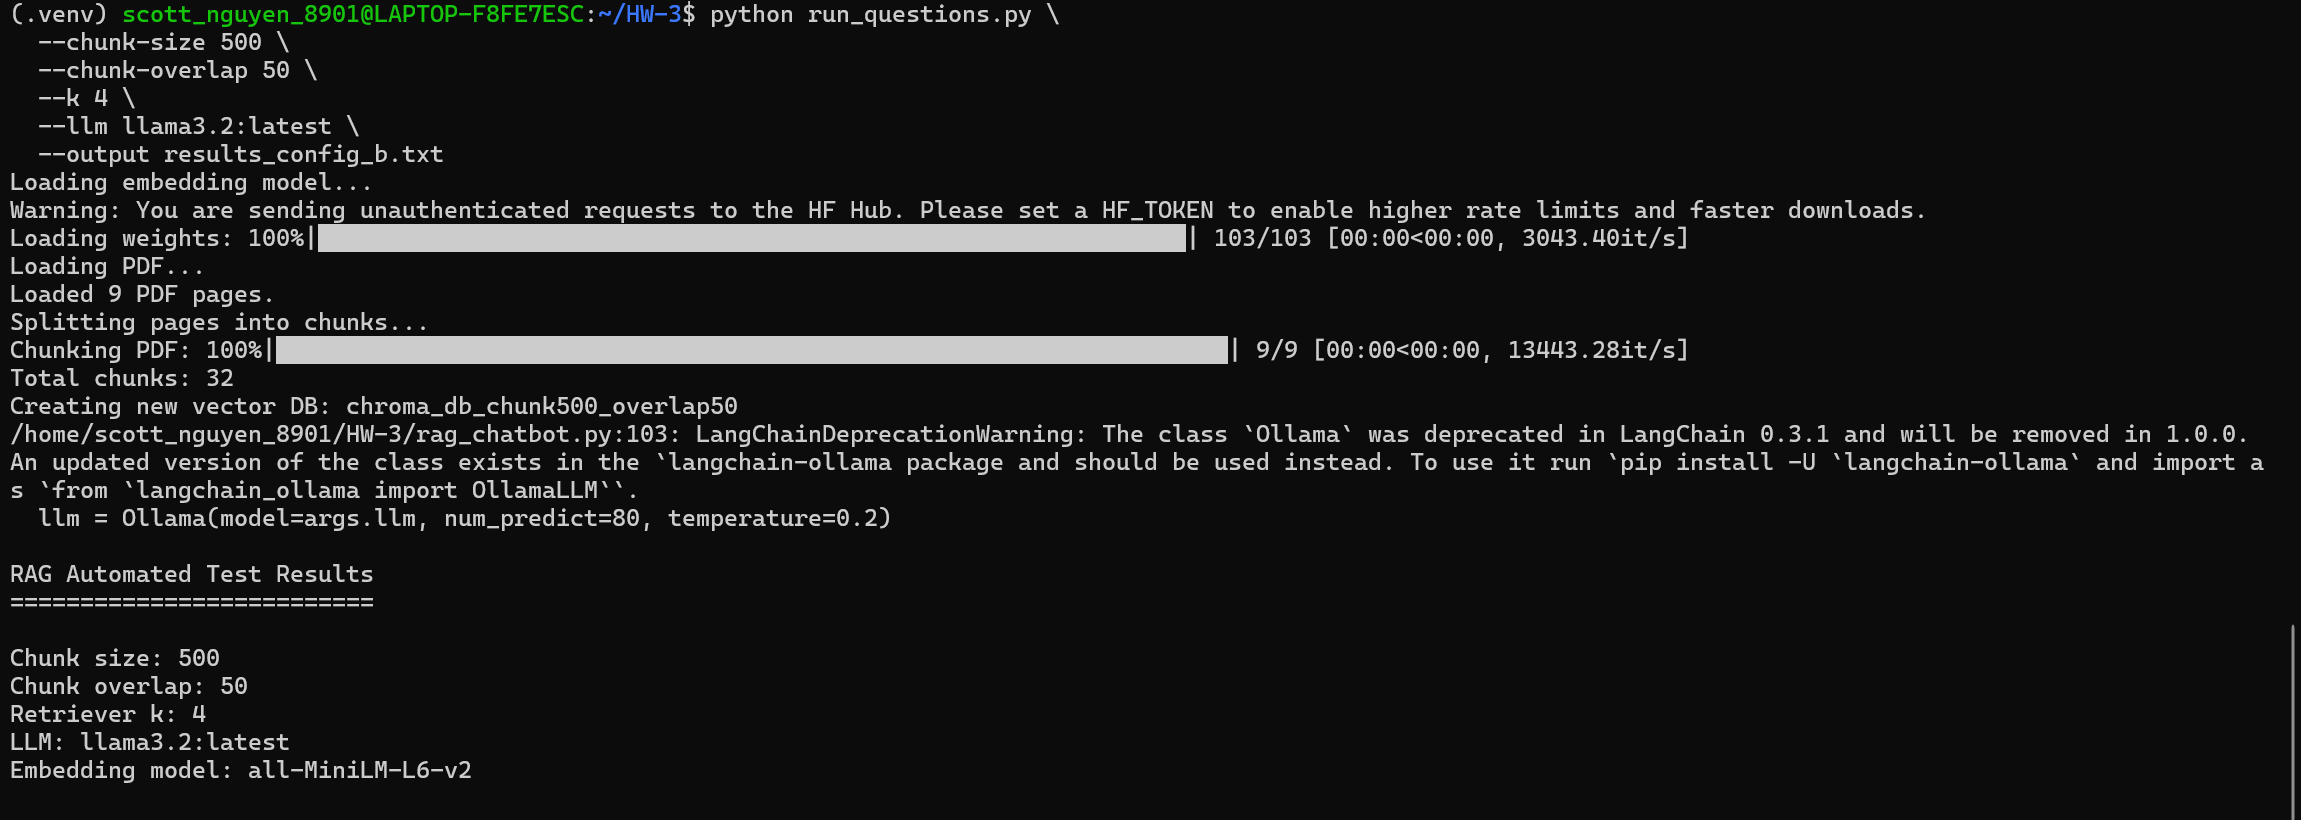
\includegraphics[width=\textwidth]{plots/0.2.png}
		\caption{Configuration B startup and chunking process.}
	\end{figure}
	
	\begin{figure}[H]
		\centering
		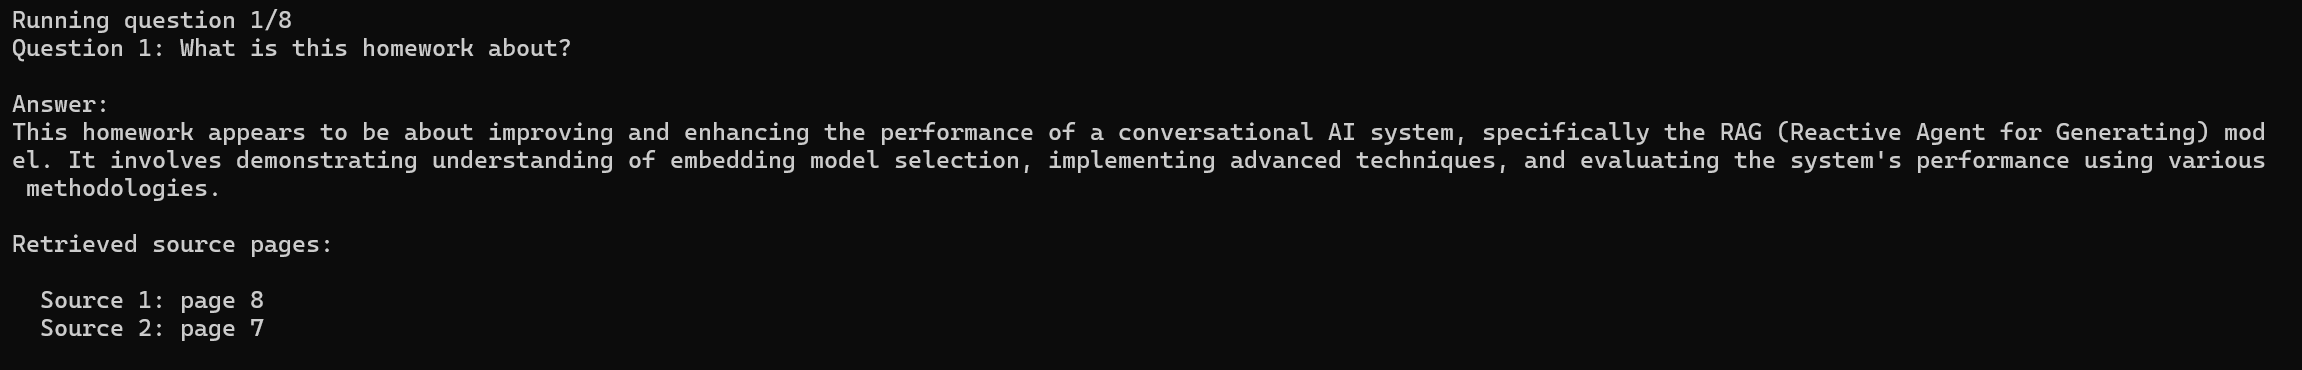
\includegraphics[width=\textwidth]{plots/1.1.png}
		\caption{Configuration A answering Question 1.}
	\end{figure}
	
	\begin{figure}[H]
		\centering
		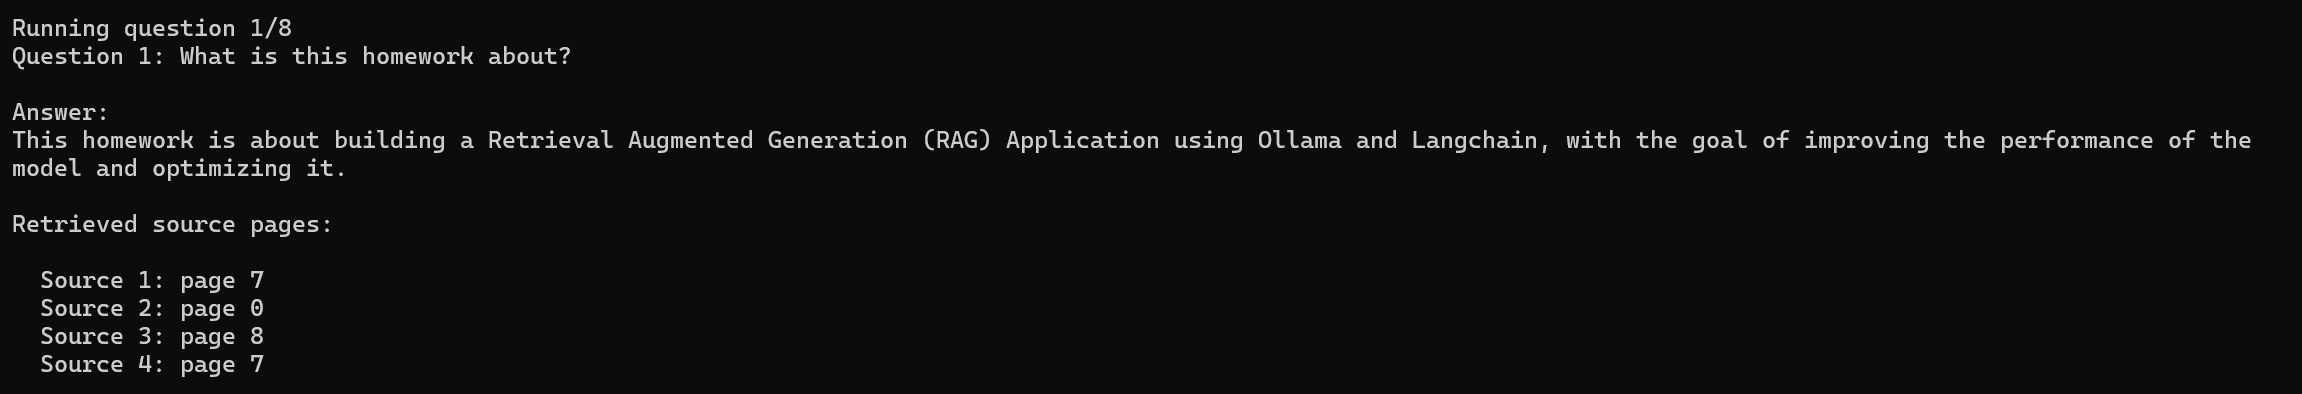
\includegraphics[width=\textwidth]{plots/1.2.png}
		\caption{Configuration B answering Question 1.}
	\end{figure}
	
	\begin{figure}[H]
		\centering
		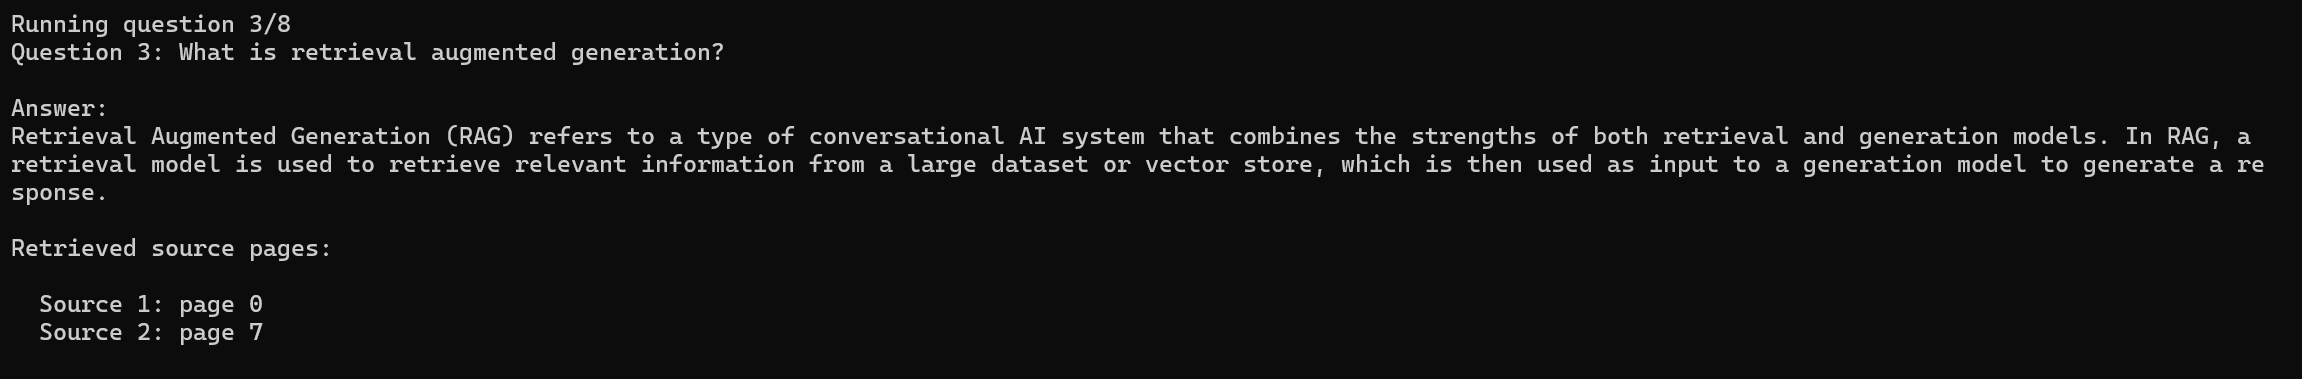
\includegraphics[width=\textwidth]{plots/3.1.png}
		\caption{Configuration A answering a RAG definition question.}
	\end{figure}
	
	\begin{figure}[H]
		\centering
		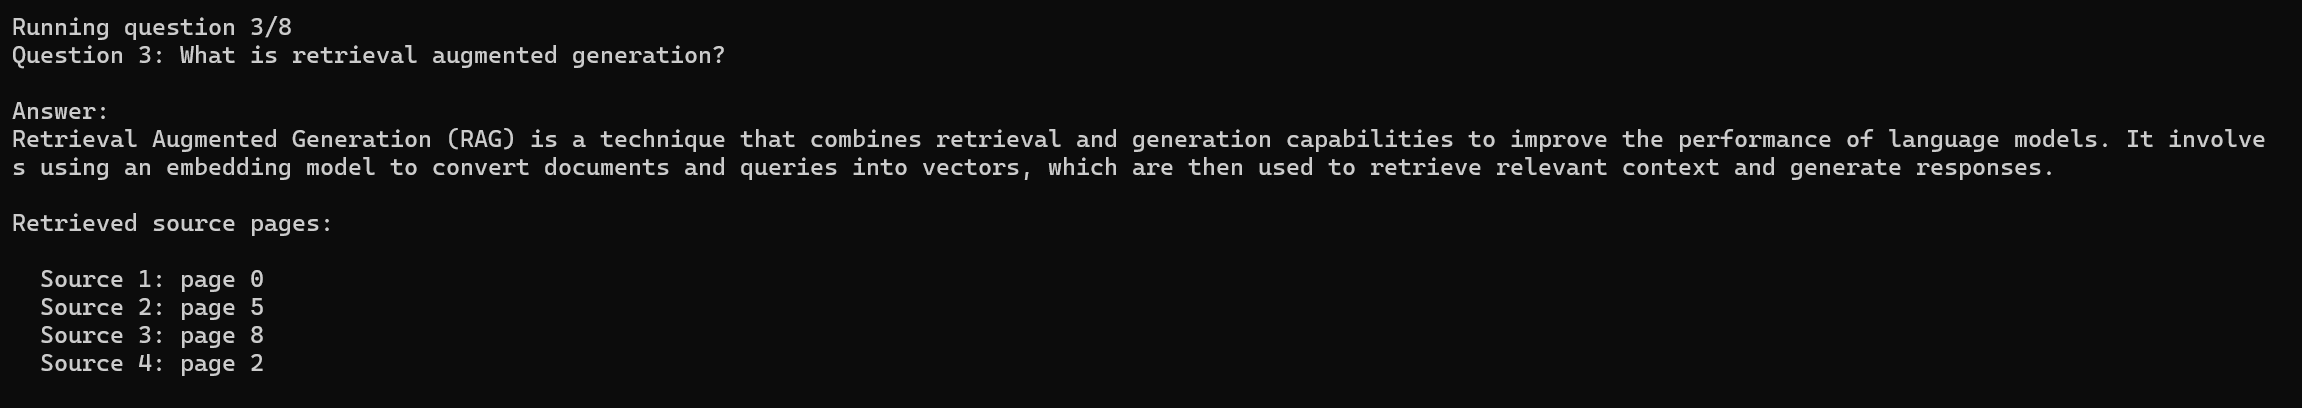
\includegraphics[width=\textwidth]{plots/3.2.png}
		\caption{Configuration B answering a RAG definition question.}
	\end{figure}
	
	\section{Log Output}
	
	The automated test script saved full responses into log files.
	
	\subsection{Configuration A Log}
	
	\lstinputlisting[
	style=terminal,
	caption={Results from Configuration A}
	]{logs/results_config_a.txt}
	
	\subsection{Configuration B Log}
	
	\lstinputlisting[
	style=terminal,
	caption={Results from Configuration B}
	]{logs/results_config_b.txt}
	
	\section{Performance Evaluation}
	
	The system was tested using eight questions covering general understanding, factual retrieval, improvement suggestions, rubric lookup, and system limitations. A negative test, ``What is the capital of France?'', was included to verify that the model restricts answers to document context.
	
	Correct behavior was to respond with ``I do not know based on the document,'' confirming proper grounding.
	
	\begin{table}[H]
		\centering
		\caption{Evaluation Question Categories}
		\begin{tabular}{ll}
			\toprule
			\textbf{Question Type} & \textbf{Purpose} \\
			\midrule
			General summary & Tests document-level understanding \\
			RAG definition & Tests conceptual explanation \\
			Embedding model & Tests specific retrieval \\
			Vector database & Tests Chroma retrieval \\
			Improvement question & Tests rubric understanding \\
			Negative test & Tests refusal for out-of-document questions \\
			\bottomrule
		\end{tabular}
	\end{table}
	
	\section{Analysis of Results}
	
	Configuration B generally produced more accurate responses due to increased context retrieval. For example, it better identified the homework as building a RAG application and correctly retrieved Chroma as the vector store. Configuration A was faster but sometimes missed relevant information because it retrieved fewer chunks.
	
	Some inconsistencies were observed in both configurations, especially when the retrieved context was incomplete. This shows that RAG quality depends on chunking, retriever settings, prompt design, and model capability.
	
	\section{Design Decisions}
	
	The embedding model \texttt{all-MiniLM-L6-v2} was selected for efficiency in a CPU-based WSL environment. The model \texttt{llama3.2:latest} provided a balance between speed and answer quality.
	
	Chroma persistence was used to avoid recomputing embeddings on every run. The automated runner was created so the same questions could be tested consistently across configurations.
	
	\section{Limitations}
	
	The system has several limitations. Retrieval quality depends on chunk size, overlap, and embedding accuracy. Smaller local models may also produce incomplete or vague responses.
	
	The system does not use re-ranking, hybrid keyword search, or advanced document filtering. It also relies on static chunking, so it may not always retrieve the most useful context for every question.
	
	\section{Future Improvements}
	
	Future work could improve the system by:
	
	\begin{itemize}
		\item Testing stronger local models such as Mistral
		\item Adding a re-ranking step after vector retrieval
		\item Improving the prompt with more structured output requirements
		\item Adding hybrid retrieval using both keyword and vector search
		\item Showing direct source snippets with each answer
	\end{itemize}
	
	\section{User Guide}
	
	Run the chatbot interactively:
	
	\begin{lstlisting}[style=terminal]
		python rag_chatbot.py --chunk-size 500 --chunk-overlap 50 --k 4 --llm llama3.2:latest
	\end{lstlisting}
	
	Run automated evaluation:
	
	\begin{lstlisting}[style=terminal]
		python run_questions.py --chunk-size 500 --chunk-overlap 50 --k 4 --llm llama3.2:latest --output logs/results_config_b.txt
	\end{lstlisting}
	
	The chatbot retrieves context, generates an answer, prints source pages, and can save results to a log file.
	
	\section{Conclusion}
	
	This project demonstrates how RAG improves answer quality by grounding responses in document context. The system successfully loaded a PDF, created embeddings, stored them in Chroma, retrieved relevant chunks, and generated answers with a local Ollama model.
	
	Smaller chunks with higher retrieval values improved accuracy, while larger chunks provided faster execution. Overall, the project showed that RAG performance depends on chunking strategy, retrieval size, prompt design, and model selection.
	
	\appendix
	
	\newpage
	
	\section{Appendix A: RAG Chatbot Source Code}
	
	\lstinputlisting[
	style=pythoncode,
	caption={rag\_chatbot.py}
	]{rag_chatbot.py}
	
	\newpage
	
	\section{Appendix B: Automated Question Runner Source Code}
	
	\lstinputlisting[
	style=pythoncode,
	caption={run\_questions.py}
	]{run_questions.py}
	
\end{document}